\documentclass{beamer}

\usepackage{amsthm}
\usepackage[utf8]{inputenc}
\usepackage[T1]{fontenc}
\usepackage[brazil]{babel}
\usepackage[export]{adjustbox}
\usepackage{listings}
\usepackage{fontspec}
\usepackage{color}

\definecolor{pblue}{rgb}{0.13,0.13,1}
\definecolor{pgreen}{rgb}{0,0.5,0}
\definecolor{pred}{rgb}{0.9,0,0}
\definecolor{pgrey}{rgb}{0.46,0.45,0.48}

\lstset{language=Java,
  showspaces=false,
  showtabs=false,
  breaklines=true,
  showstringspaces=false,
  breakatwhitespace=true,
  commentstyle=\color{pgreen},
  keywordstyle=\color{pblue},
  stringstyle=\color{pred},
  basicstyle=\ttfamily,
}


\usetheme{Madrid}
\usecolortheme{beetle}
\usefonttheme{professionalfonts}

\setmainfont{Oswald}

\lstset{basicstyle=\ttfamily,breaklines=true}
\beamertemplatenavigationsymbolsempty

\begin{document}

\selectlanguage{brazil}
\title[Listas]{Listas}
\author{Prof. Andrey Masiero}

\begin{frame}[plain,noframenumbering]
  \titlepage
\end{frame}

\begin{frame}[plain,noframenumbering]
  \frametitle{Agenda}
  \tableofcontents
\end{frame}

\section{Lista}

\begin{frame}
	\begin{center}
        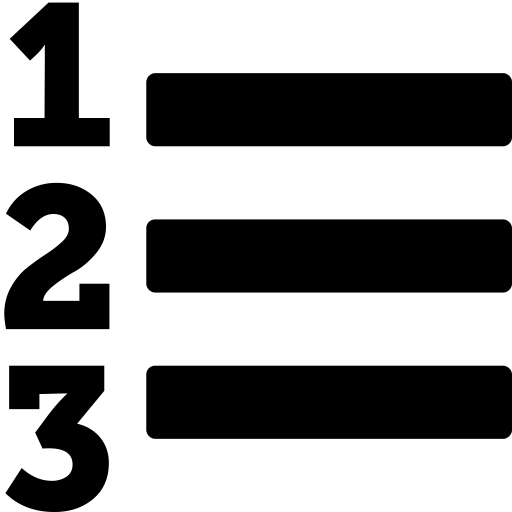
\includegraphics[scale=0.2]{images/list.png}

		\Huge Lista
	\end{center}
\end{frame}

\begin{frame}
	\frametitle{Lista Sequencial}
    \begin{table}
        \caption{Operações básicas de Lista}
        \label{tab:lista}
        \begin{tabular}{| c | c |}
            \hline
            Operação & Descrição \\ \hline
            \texttt{add} & Adiciona um novo elemento na lista \\ \hline
            \texttt{remove} & Remove um valor da lista a partir da posição \\ \hline
            \texttt{get} & Encontra a posição de um determinado número na lista \\ \hline
            \texttt{size} & Consulta quantos elementos estão armazenados na lista \\ \hline
            \texttt{isEmpty} & Consulta se a lista está vazia\\ \hline
        \end{tabular}
    \end{table}
\end{frame}

\begin{frame}
	\frametitle{add}
    \centering
    \lstinputlisting[language=Java]{src/add.java}
\end{frame}

\begin{frame}
	\frametitle{get}
    \centering
    \lstinputlisting[language=Java]{src/get.java}
\end{frame}

\begin{frame}
	\frametitle{remove}
    \centering
    \lstinputlisting[language=Java]{src/remove.java}
\end{frame}

\begin{frame}
	\frametitle{isEmpty}
    \centering
    \lstinputlisting[language=Java]{src/vazio.java}
\end{frame}

\begin{frame}
	\frametitle{size}
    \centering
    \lstinputlisting[language=Java]{src/size.java}
\end{frame}

\section{Exercícios}

\begin{frame}
    \frametitle{Exercícios}
    \begin{enumerate}
        \item Implemente uma Lista utilizando vetor (sequencial/estática).
        \item Implemente uma Lista utilizando vetor (encadeada/dinâmica).
        \item Faça um programa que teste todas as estruturas criadas.
    \end{enumerate}
\end{frame}

\section{Referências}

\begin{frame}
    \frametitle{Referências Bibliográficas}
    \begin{enumerate}
        \item Cormen, Thomas H., Charles E. Leiserson, Ronald L. Rivest, and Clifford Stein. ``Introduction to algorithms second edition.'' (2001).
        \item Tamassia, Roberto, and Michael T. Goodrich. ``Estrutura de Dados e Algoritmos em Java.'' Porto Alegre, Ed. Bookman 4 (2007).
        \item Ascencio, Ana Fernanda Gomes, and Graziela Santos de Araújo. ``Estruturas de Dados: algoritmos, análise da complexidade e implementações em JAVA e C/C++.'' São Paulo: Perarson Prentice Halt 3 (2010).
    \end{enumerate}
\end{frame}

\end{document}
